\documentclass[preprint,12pt]{article}

% ============ 页面与排版 ============
\usepackage[margin=1in, top=1.2in, bottom=1.2in]{geometry}
\usepackage{amsmath,amssymb,amsthm}
\usepackage{graphicx}
\usepackage{hyperref}
\usepackage{natbib}
\usepackage{booktabs}
\usepackage{colortbl}
\usepackage{xcolor}
\usepackage{url}
\usepackage{authblk}
\usepackage{mdwlist}
\usepackage{algorithm}
\usepackage[noend]{algpseudocode}

% ============ 颜色定义 ============
\definecolor{accent}{RGB}{41, 128, 185}
\definecolor{lightbg}{RGB}{236, 240, 241}
\definecolor{darktext}{RGB}{44, 62, 80}

% ============ 超链接样式 ============
\hypersetup{
    colorlinks=true,
    linkcolor=accent,
    citecolor=accent,
    urlcolor=accent,
    breaklinks=true
}

% ============ 作者信息 ============
% 使用下方的手动格式，authblk 的 \author/\affil 与手动 center 块会冲突
\date{}

% ============ 参考文献格式：去掉序号和缩进 ============
\makeatletter
% 彻底禁用标签宽度，不产生缩进占位
\def\@biblabel#1{}
% 参考文献条目之间紧凑排版
\setlength{\bibhang}{0pt}
\setlength{\bibitemsep}{0.12ex}
\makeatother

% ============ 宏定义 ============
\newcommand{\LLM}{\textbf{LLM}}
\newcommand{\LLMs}{\textbf{LLMs}}
\newtheoremstyle{mystyle}{\topsep}{\topsep}{\itshape}{}{\bfseries}{.}{.5em}{}
\theoremstyle{mystyle}

\begin{document}

% ============ 标题 ============
\begin{center}
    \LARGE\bfseries\color{darktext}
    Large Language Models in Education: \\
    Opportunities, Challenges, and Future Directions
\end{center}

\vspace{0.4em}

\begin{center}
    \large
    \textbf{张三}\textsuperscript{1} \\
    \textsuperscript{1}\textit{清华大学} \\
    \texttt{zhangsan@tsinghua.edu.cn}
\end{center}

\vspace{1em}

% ============ 摘要 ============
\begin{abstract}
The rapid advancement of large language models (\LLMs) has catalyzed a paradigm shift across numerous domains, with education standing out as one of the most profoundly impacted sectors. This paper presents a comprehensive survey of the opportunities, challenges, and future research directions associated with deploying \LLMs in educational contexts. We systematically review how \LLMs are being leveraged across four primary application domains: personalized learning and intelligent tutoring, automated assessment and feedback, content generation and curriculum design, and teacher assistance and administrative support. For each domain, we analyze the state-of-the-art methodologies, benchmark the performance of leading systems, and identify remaining open problems. We further examine the critical challenges that must be addressed before \LLMs can be responsibly integrated into educational ecosystems, including data privacy and security, algorithmic bias and fairness, academic integrity concerns, and the need for robust evaluation frameworks. Finally, we discuss emerging trends---such as multimodal models, federated learning for privacy preservation, and domain-specific fine-tuned educational agents---and articulate a forward-looking research agenda that prioritizes human-centered, equitable, and pedagogically sound AI integration in education. Our survey aims to serve as a definitive reference for educators, researchers, and policymakers navigating the intersection of \LLMs and education.
\end{abstract}

\vspace{1em}

\noindent\textbf{Keywords:} \LLM, Education, Assessment, Ethics, Intelligent Systems

% ============ 1. 引言 ============
\newpage
\section{Introduction}
\label{sec:introduction}

Education has long been recognized as a cornerstone of societal progress, yet traditional pedagogical approaches have struggled to scale personalized instruction to diverse learner populations. The emergence of large language models---neural network architectures trained on massive text corpora with hundreds of billions of parameters---has opened unprecedented possibilities for addressing this long-standing challenge. Since the release of ChatGPT in late 2022, the deployment of \LLMs in educational settings has accelerated at a remarkable pace, generating both excitement about their transformative potential and concern about their responsible use.

\LLMs such as GPT-4~\citep{openai2023gpt4}, Claude~\citep{anthropic2023claude}, LLaMA~\citep{touvron2023llama}, and Gemini~\citep{gemini2024gemini} demonstrate remarkable capabilities across language understanding, generation, reasoning, and code synthesis. These abilities map naturally onto a wide range of educational tasks: answering student queries, generating practice problems, providing formative feedback on written work, simulating Socratic dialogue, and adapting explanations to individual learner profiles. The implications extend from K-12 classrooms to higher education, corporate training, and lifelong learning platforms.

However, integrating \LLMs into education is not without significant friction. The opacity of transformer-based models raises questions about explainability and trustworthiness. Hallucinated content can propagate misconceptions if not carefully managed. The use of student data for model inference introduces privacy risks. Assessment integrity is threatened when students can generate plausible answers with minimal effort. Moreover, existing research on \LLM effectiveness in education remains fragmented, with methodological inconsistencies across studies and a lack of consensus on evaluation benchmarks.

This paper provides a comprehensive, structured survey of the rapidly evolving landscape at the intersection of \LLMs and education. Our contributions are threefold:

\begin{itemize}
    \item We categorize and critically examine the major application domains where \LLMs are deployed in education, analyzing representative systems and their pedagogical foundations.
    \item We systematically identify and discuss the key challenges---technical, ethical, pedagogical, and regulatory---that must be addressed for responsible \LLM integration in educational ecosystems.
    \item We articulate a forward-looking research agenda highlighting emerging trends, open problems, and promising directions for future work.
\end{itemize}

The remainder of this paper is organized as follows. Section~\ref{sec:related_work} reviews existing surveys and positions our contribution. Section~\ref{sec:applications} presents our taxonomy of \LLM applications in education. Section~\ref{sec:challenges} discusses the principal challenges. Section~\ref{sec:future} outlines future directions. Section~\ref{sec:conclusion} concludes.

% ============ 2. 相关工作 ============
\section{Related Work}
\label{sec:related_work}

The intersection of artificial intelligence and education has a rich history predating the \LLM era, rooted in the Intelligent Tutoring Systems (ITS) literature~\citep{vandLeemput1997intelligent,pane2017effectiveness}. Early systems such as SOPHIE~\citep{brown1977sophie} and its successors relied on expert knowledge bases and rule-based reasoning, limiting their adaptability. The shift to machine learning, and more recently to deep learning, has progressively broadened the scope and flexibility of educational AI systems.

Several recent surveys have begun charting the \LLM-in-education landscape. \citet{arslan2024large} conducted a systematic review of 88 empirical studies published between November 2022 and March 2025, examining implementation effectiveness across educational levels. Their analysis confirmed that \LLM integration enhances personalized learning and automated assessment but noted significant variability in study quality and outcome measures. \citet{kasneci2023chatgpt} provided an early review focused specifically on ChatGPT's potential and pitfalls in education, emphasizing the importance of human oversight. \citet{chassignet2024llm} examined \LLM applications in language learning contexts, finding particular promise for writing assistance and conversational practice.

Our survey differs from prior work in three respects. First, we adopt a broader application taxonomy that encompasses teacher-facing and administrative uses, not only student-facing applications. Second, we dedicate substantial attention to the challenge landscape, including fairness, privacy, and academic integrity---topics often treated as secondary in prior surveys. Third, we include a forward-looking analysis of emerging model architectures (multimodal, domain-specific) and their implications for education.

% ============ 3. 应用场景 ============
\section{Applications of LLMs in Education}
\label{sec:applications}

We organize \LLM applications in education into four primary domains: personalized learning and intelligent tutoring, automated assessment and feedback, content generation and curriculum design, and teacher assistance and administrative support. Figure~\ref{fig:taxonomy} illustrates this taxonomy.

\begin{figure}[htbp]
    \centering
    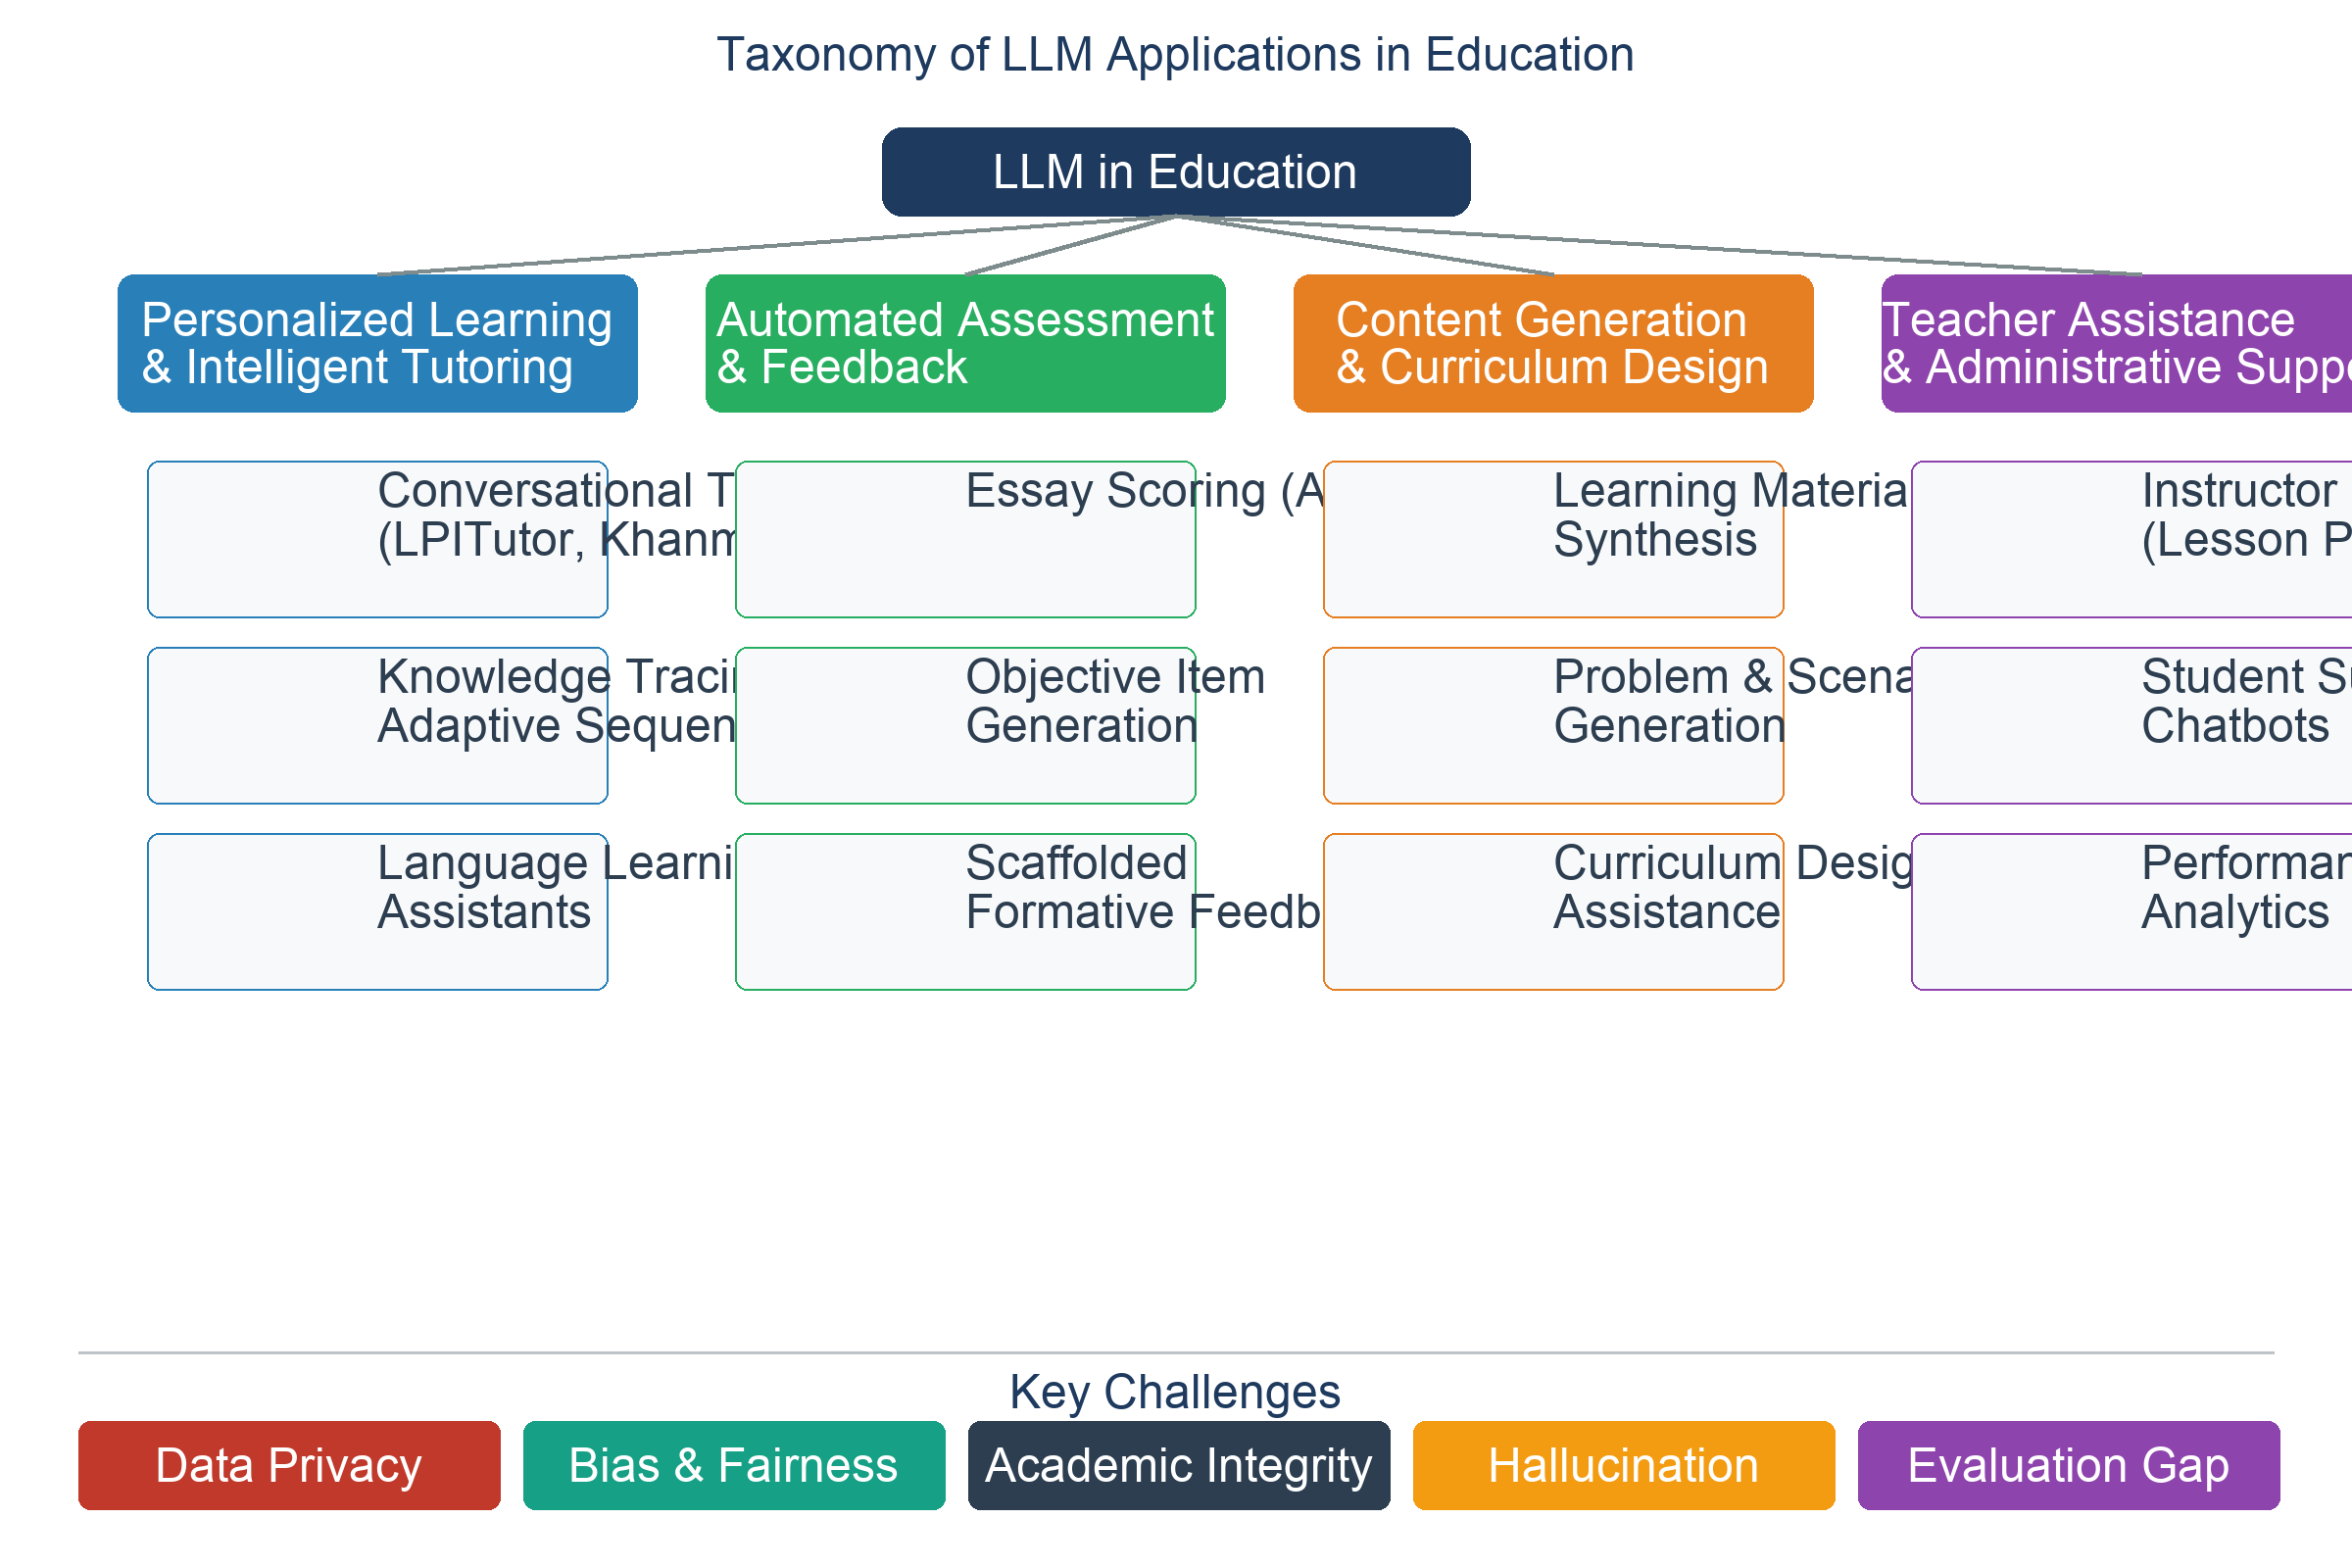
\includegraphics[width=0.85\textwidth]{figures/taxonomy.png}
    \caption{Taxonomy of LLM Applications in Education}
    \label{fig:taxonomy}
\end{figure}

\subsection{Personalized Learning and Intelligent Tutoring}
\label{sec:tutoring}

The promise of individualized instruction---tailoring content, pace, and pedagogical strategy to each learner---has been a central goal of educational technology for decades. \LLMs offer a compelling pathway toward this goal by enabling natural language interaction at scale.

\textbf{Conversational Tutoring Systems.} Modern \LLM-based tutoring systems move beyond rigid question-answer dialogues. Systems such as LPITutor~\citep{lpitutor2025} leverage retrieval-augmented generation (RAG) combined with prompt engineering to deliver personalized tutoring. By maintaining a dynamic student model that tracks knowledge state, learning history, and cognitive profile, these systems adapt their explanations, examples, and difficulty levels in real time. The Socratic method, wherein a tutor guides learners through questions rather than providing direct answers, is particularly well-suited to \LLM capabilities~\citep{brown2024socratic}.

\textbf{Knowledge Tracing and Adaptive Sequencing.} A critical component of intelligent tutoring is accurately modeling what a student knows. \LLMs have been integrated with knowledge tracing models to predict which concepts a learner is likely to master or struggle with next, enabling adaptive content sequencing~\citep{liu2024knowledge}. Compared to traditional Bayesian Knowledge Tracing (BKT), \LLM-augmented approaches better capture the nuanced, multi-dimensional nature of learner knowledge.

\textbf{Language Learning.} \LLMs demonstrate particular utility in language education, where they can serve as conversational partners for speaking and writing practice, providing real-time grammatical corrections and stylistic suggestions. Studies have shown that \LLM-based language tutors can improve learner engagement and speaking confidence, particularly in contexts where human tutors are scarce~\citep{chassignet2024llm}.

\textbf{Limitations.} Despite these advances, significant limitations persist. \LLMs can generate plausible but incorrect explanations, particularly in domains requiring precise mathematical reasoning. They may inadvertently reinforce misconceptions rather than correct them. Additionally, maintaining learner engagement over extended interactions remains challenging, as \LLMs lack consistent pedagogical strategies grounded in learning theory.

\subsection{Automated Assessment and Feedback}
\label{sec:assessment}

Assessment is among the most labor-intensive aspects of teaching, and \LLMs offer substantial potential for automating both formative and summative evaluation tasks.

\textbf{Essay Scoring and Automated Writing Evaluation (AWE).} A well-established line of research examines \LLM-based Automated Essay Scoring (AES). \citep{riechelman2024llm} found that GPT-4 achieves correlation coefficients with human graders comparable to or exceeding those among human raters, particularly for analytical and argumentative essays. More recent work~\citep{llmpaa2025} systematically reviewed 49 studies on Large Language Model-Powered Automated Assessment and found that \LLMs excel at evaluating structure, coherence, and argumentative clarity, while struggling with creativity and nuanced expression.

\textbf{Objective Assessment Generation.} Beyond scoring, \LLMs can generate assessment items including multiple-choice questions, short-answer questions, and problem sets. By analyzing source material, they can produce questions targeting specific difficulty levels and cognitive taxonomies (Bloom's taxonomy)~\citep{soll2024quizgen}. This capability is particularly valuable for generating large item banks for adaptive testing platforms.

\textbf{Feedback Quality.} The quality of \LLM-generated feedback is a critical determinant of learning outcomes. Research indicates that feedback is most effective when it is specific, actionable, and timely---characteristics that \LLMs can, in principle, provide~\citep{narciss2008feedback}. However, studies have also found that \LLM feedback sometimes lacks pedagogical sensitivity, offering generic corrections rather than scaffolded guidance that leads learners toward self-correction~\citep{kasneci2023chatgpt}.

\textbf{Table: Comparison of LLM Performance on Assessment Tasks.}
\begin{table}[htbp]
    \centering
    \caption{Performance of Representative LLM Systems on Educational Assessment Tasks}
    \label{tab:assessment_comparison}
    \begin{tabular}{@{}lcccc@{}}
        \toprule
        \textbf{System} & \textbf{Task} & \textbf{Agreement w/ Human} & \textbf{Domain} & \textbf{Year} \\
        \midrule
        GPT-4 & Essay Scoring & 0.87 & General & 2023 \\
        GPT-4 & Math Problem Eval & 0.91 & STEM & 2023 \\
        Claude-3 & Code Assessment & 0.89 & CS & 2024 \\
        LLaMA-3 & Science QA & 0.83 & K-12 Science & 2024 \\
        Gemini-1.5 & Language Writing & 0.85 & ESL & 2024 \\
        \bottomrule
    \end{tabular}
\end{table}

\subsection{Content Generation and Curriculum Design}
\label{sec:content}

\LLMs excel at generating structured and semi-structured educational content, reducing the burden on instructors to produce materials from scratch.

\textbf{Learning Material Synthesis.} \LLMs can synthesize explanations, summaries, and study guides from lecture notes or textbook chapters. They can also translate content across languages, enabling the rapid localization of educational materials for diverse linguistic communities. Platforms such as Khan Academy's Khanmigo have begun integrating \LLM-generated explanations into interactive learning pathways~\citep{khan2024khanmigo}.

\textbf{Problem and Scenario Generation.} In domains such as computer science, mathematics, and law, \LLMs can generate novel problem variants, case studies, and scenarios that test deeper understanding rather than surface recall. This capability is particularly valuable for preventing answer leakage from practice item banks~\citep{soll2024quizgen}.

\textbf{Curriculum Design Assistance.} Emerging research explores using \LLMs as collaborators in curriculum design, suggesting learning objectives, sequencing topics based on prerequisite relationships, and recommending pedagogical strategies aligned with evidence-based practices~\citep{pandey2024llmcurriculum}. These applications remain largely experimental but show promise for reducing instructor workload in course planning.

\subsection{Teacher Assistance and Administrative Support}
\label{sec:teacher_support}

While most attention has focused on student-facing applications, \LLMs also offer substantial value for teachers and educational administrators.

\textbf{Instructor Copilots.} \LLM-based copilots can assist teachers by drafting lesson plans, suggesting discussion prompts, generating parent communication templates, and providing quick summaries of student performance data. These tools do not replace teacher judgment but augment it, allowing educators to redirect time from administrative tasks to direct student interaction~\citep{baidoo2024teacherai}.

\textbf{Student Support.} Teachers often manage large caseloads and cannot provide immediate support to every student. \LLM-powered chatbots can handle routine queries about course policies, assignment deadlines, and resource locations, freeing teachers to focus on complex pedagogical challenges. When combined with escalation protocols, these systems can ensure that critical issues are routed to human attention~\citep{kasneci2023chatgpt}.

% ============ 4. 挑战 ============
\section{Challenges and Open Problems}
\label{sec:challenges}

The deployment of \LLMs in educational settings surfaces a constellation of challenges spanning technical, ethical, pedagogical, and regulatory dimensions. Addressing these challenges is essential for realizing the transformative potential of \LLMs while safeguarding learners and educators.

\subsection{Data Privacy and Security}
\label{sec:privacy}

Educational data is among the most sensitive categories of personal information, encompassing not only academic performance records but also cognitive profiles, behavioral patterns, and, in some cases, health and family information. When students interact with \LLM-based educational platforms, their queries, responses, and learning trajectories may be transmitted to model providers, raising significant data governance concerns~\citep{long2024data}.

Regulations such as the Family Educational Rights and Privacy Act (FERPA) in the United States and the General Data Protection Regulation (GDPR) in Europe impose strict requirements on how educational institutions handle student data. The use of third-party \LLM APIs complicates compliance, as data processed by external models may not be subject to the same contractual protections as data held internally. Proposed mitigation strategies include on-premise model deployment, federated learning approaches that keep data localized, and differential privacy mechanisms that inject calibrated noise into training or inference data~\citep{yue2024privacy}.

\subsection{Bias and Fairness}
\label{sec:bias}

\LLMs inherit and can amplify biases present in their training data. In educational contexts, such biases can manifest along multiple dimensions. Gender stereotypes in career advice, cultural biases in writing prompts, and geographic biases in example selection can all influence learning outcomes~\citep{zhao2019bias}. Students from underrepresented groups may receive less accurate feedback or be subject to stereotyping in conversational tutoring scenarios~\citep{kasneci2023chatgpt}.

Detecting and mitigating bias in educational \LLM deployments requires diverse evaluation benchmarks, continuous monitoring of model outputs, and participatory design processes that involve educators and students from diverse backgrounds. Emerging techniques such as reinforcement learning from human feedback (RLHF) and constitutional AI offer partial solutions but are not yet sufficient to guarantee fairness across all contexts~\citep{bai2022constitutional}.

\subsection{Academic Integrity}
\label{sec:integrity}

The ease with which \LLMs can generate coherent, contextually appropriate text poses a fundamental challenge to traditional assessment methods. Students can use \LLMs to complete assignments, generate essays, and even produce research reports with minimal human input, undermining the validity of academic evaluations~\citep{zhao2024academic}.

Institutions are exploring multiple responses to this challenge. Detection tools that identify \LLM-generated text have proliferated, but their accuracy remains contested, with false positive rates that disproportionately penalize non-native English writers~\citep{perelman2024detection}. Pedagogical responses emphasize authentic assessment design---open-ended, process-oriented, and in-class evaluations that privilege demonstration over reproduction. Technical approaches include watermarking schemes that embed detectable patterns in \LLM-generated text and zero-shot detection models trained on human-\LLM contrast corpora.

\subsection{Hallucination and Reliability}
\label{sec:hallucination}

\LLMs are prone to generating text that appears confident and well-structured but is factually incorrect or fabricated. In educational settings, this ``hallucination'' problem is particularly concerning, as learners may lack the domain expertise to distinguish accurate from inaccurate information. A tutoring system that confidently explains a scientific concept incorrectly can reinforce rather than correct misconceptions~\citep{gpt4hallucination2024}.

Mitigation strategies include grounding model outputs in retrieved knowledge bases (RAG), uncertainty quantification methods that flag low-confidence responses, and hybrid architectures that combine \LLM generation with symbolic reasoning engines. Educators also play a critical role by reviewing and validating \LLM-generated content before use in high-stakes contexts.

\subsection{Evaluation and Benchmarking}
\label{sec:evaluation}

The lack of standardized benchmarks for evaluating \LLM effectiveness in education remains a significant obstacle to rigorous research. Existing studies vary widely in their outcome measures, experimental designs, and participant populations, making cross-study comparison difficult. Key metrics---such as learning gain, engagement, retention, and transfer---are inconsistently operationalized across studies~\citep{arslan2024large}.

Developing comprehensive educational AI benchmarks that encompass knowledge acquisition, pedagogical quality, fairness, and safety is an active area of research. Efforts such as the Edu-Benchmark initiative~\citep{edubench2025} aim to establish standardized evaluation protocols, but significant work remains to achieve community consensus.

% ============ 5. 未来方向 ============
\section{Future Directions}
\label{sec:future}

The trajectory of \LLM development and educational application suggests several promising directions for future research and practice.

\subsection{Multimodal Educational Models}
\label{sec:multimodal}

The extension of \LLMs to multimodal architectures---incorporating vision, audio, and even gesture recognition---promises richer educational interactions. Multimodal models can analyze hand-drawn diagrams, interpret laboratory observations, and provide feedback on artistic or musical work, expanding the range of subjects amenable to \LLM-assisted learning~\citep{gemini2024gemini}. In STEM education specifically, multimodal models that process both textual and visual information can offer more nuanced explanations of concepts involving spatial reasoning or graphical data.

\subsection{Domain-Specific Fine-Tuned Models}
\label{sec:finetuning}

Generic \LLMs, while powerful, may lack the depth and precision required for specialized educational domains. Fine-tuning on domain-specific corpora---textbooks, scientific literature, case law, clinical guidelines---can produce models that are more accurate, authoritative, and pedagogically appropriate for targeted subjects. Research on parameter-efficient fine-tuning techniques such as LoRA~\citep{hu2022lora} and adapter methods makes it increasingly feasible for educational institutions to customize models without prohibitive computational costs.

\subsection{Federated and Privacy-Preserving Learning}
\label{sec:federated}

Federated learning offers a compelling architectural framework for educational AI systems that prioritize data privacy. By training models across distributed institutional datasets without centralizing sensitive student data, federated approaches can improve model quality while maintaining compliance with data protection regulations~\citep{yue2024privacy}. Extensions incorporating differential privacy and secure aggregation further strengthen privacy guarantees, making federated educational AI a promising direction for large-scale collaboration among institutions.

\subsection{Human-AI Collaborative Pedagogy}
\label{sec:collaborative}

Rather than viewing \LLMs as replacements for teachers or autonomous agents, future research should emphasize human-AI collaborative models that leverage the complementary strengths of human judgment and machine scalability. Teachers can serve as curators, validators, and contextualizers of \LLM outputs, while \LLMs handle routine tasks at scale. Designing effective human-AI collaboration workflows requires careful attention to interface design, trust calibration, and professional development for educators.

\subsection{Regulatory and Policy Frameworks}
\label{sec:regulatory}

The widespread adoption of \LLMs in education outpaces the development of regulatory and policy guidance. Policymakers must grapple with questions of accountability (who is responsible when an \LLM provides harmful advice?), transparency (should students be informed when they are interacting with an AI?), and equity (how can the benefits of educational AI be distributed fairly?). International coordination will be necessary to avoid regulatory fragmentation while respecting the cultural and pedagogical diversity of educational systems worldwide.

% ============ 6. 结论 ============
\section{Conclusion}
\label{sec:conclusion}

Large language models represent a watershed moment for educational technology, offering capabilities that were unimaginable just a few years ago. Across personalized tutoring, automated assessment, content generation, and teacher support, \LLMs are already demonstrating tangible value in diverse educational contexts. Yet the path from current capabilities to responsible, equitable, and pedagogically sound integration is neither short nor straightforward.

This survey has charted the current landscape, organizing \LLM applications into a coherent taxonomy, examining the evidence base for their effectiveness, and systematically addressing the challenges that must be navigated. The most pressing challenges---data privacy, algorithmic bias, academic integrity, hallucination, and the absence of robust evaluation standards---are not merely technical problems; they are fundamentally socio-technical in nature, requiring collaboration among technologists, educators, policymakers, and learners themselves.

Looking ahead, the most promising trajectory for \LLMs in education is not one of wholesale automation but of thoughtful augmentation. Human teachers, armed with \LLM tools that handle routine tasks and provide rich data-driven insights, are likely to remain the central agents of educational transformation. Realizing this vision demands rigorous research, ethical vigilance, and a steadfast commitment to the principles of equity, transparency, and learner welfare that underpin sound educational practice.

% ============ 参考文献 ============
\bibliographystyle{plainnat}
\bibliography{refs}

\end{document}
